%==== Document Setup (usthesis)======================================
\documentclass[report,                       %... Document type
               12pt,oneside,openany,a4paper, %... Layout
               report, a5block,          	%... A5 type block
               afrikaans, english,            %... Afrikaans default language
               ]{usthesis}
               
%==== Language setup ================================================
\usepackage[latin1]{inputenc}%................... Recognizes �, �, etc
\usepackage{babel}%.............................. Language setup

%==== Math setup ====================================================
% \usepackage{amsmath}%............................ Advanced
 % math (before fonts) \usepackage{amssymb}%............................ AMS Symbol fonts

%==== Font setup (default is Computer Modern) =======================
 \usepackage[T1]{fontenc}%........................ Type 1 fonts
 \usepackage{textcomp}%........................... Additional text character
 \usepackage{bm}%................................. Bold math symbols (after fonts)
 
 %==== Ref's, Bib's and Nomencl ======================================
 \usepackage{usnomencl}%.......................... List of symbols (in usthesis pack)
 \usepackage{usbib}%.............................. Bibliography    (in usthesis pack)
    \bibliographystyle{usmeg-a}
    \renewcommand\bibfont{\small}

    %% For usmeg-a, the bib is a list of references. If you
    %% are using usmeg-n comment out the following lines
    \addto{\captionsafrikaans}{\renewcommand{\bibname}{Lys van Verwysings}}
    \addto{\captionsenglish}{\renewcommand{\bibname}{List of References}}
    
    %==== Graphics and Color ============================================
\usepackage{graphicx}%........................... Graphicx loaded in usthesis
\usepackage{color}%.............................. Color setup

%==== Additional USthesis packages ==================================

\usepackage{ussummary}%.......................... Mech Eng summary page (in usthesis pack)

%==== Local Defs ====================================================
\makeatletter

\usepackage{epstopdf}
%
% Please insert user defined commands here
% and NOT in the document itself!
%

\makeatother
%==== Title Page ====================================================

\title{Development of Cashless Vending Machine}

\author{JC\ Lock}
       {JC Lock \\16016548}

\subject{Mechatronic Project 488}
        {Mechatronic Project 488}

\ReportDescript{Final Report}

\address{Department of Mechanical and Mechatronic Engineering,\\
         Stellenbosch University,\\
         Private Bag X1, Matieland 7602.}

\studyleader{Prof. G-J van Rooyen}

\setdate{9}{2013}

\begin{document}

\frontmatter%========================================================

%\TitlePage
%\CopyrightPage
%\chapter{Declaration}

I, the undersigned, hereby declare that the work contained within this report is my own, original work.\par
\vspace{1.5cm}

\noindent%
\parbox{.5\textwidth}{%
  Handtekening:\quad\dotfill\par
  \hfill JC\ Lock\hspace{1.2cm}\null}\vspace{1cm}
\newline

\vspace{1.5cm}
\noindent%
\parbox{.5\textwidth}{%
  Datum:\quad\dotfill\par}

%%*** Summary Heading ************************************************

\begin{Summary}{Mechatronic Project 488: Summary}

   \noindent
   \begin{tabular}{@{}ll@{}}
      \textsf{Student:}    &  JC\ Lock\\
      \textsf{Co-worker:} &
   \end{tabular}

%*** The Summary table **********************************************
\begin{SumTable}
 \hline%=============================================================
 \SumHead{Title of Project}\\
 \hline%=============================================================
 Development of Cashless Vending Machine.
 \\

 \hline%=============================================================
 \SumHead{Objectives}\\
 \hline%=============================================================
 Program and make a model vending machine which acceepts payments made via a cellphone.
 \\

 \hline%=============================================================
 \SumHead{Which aspects of the project are new/unique?}\\
 \hline%=============================================================
 The easy use of simple cellphone technologies most students currently have built into in their
 cellphones, such as NFC and QR Codes.
 \\
   
 \hline%=============================================================
 \SumHead{What are the findings?}\\
 \hline%=============================================================
 A working test model was built which accepts faux money paid with either QR Codes or NFC. All
 the necessary security measures, i.e. encryption and challenges, were added as well as a
 central web server that tracks user transactions.
 \\

 \hline%=============================================================
 \SumHead{What value do the results have?}\\
 \hline%=============================================================
 The results show that the machine is working reliably. Some improvements can be made, but the
 overall machine is working as expected.
 \\

 \hline%=============================================================
 \SumHead{If more than one student is involved, what is each one's contribution?}\\
 \hline%=============================================================
 N/A
 \\

 \hline%=============================================================
 \SumHead{Which aspects of the project will carry on after completion?}\\
 \hline%=============================================================
 
 \\

 \hline%=============================================================
 \SumHead{What are the expected advantages of continuation?}\\
 \hline%=============================================================
 
 \\

 \hline%=============================================================
 \SumHead{What arrangements have been made to expedite continuation?}\\
 \hline%=============================================================
 
 \\

 \hline%=============================================================
\end{SumTable}

%*** Signatures *****************************************************

\vspace{1.5cm}
\SumSignatures

\end{Summary}

\endinput

%\begin{abstract}
   
   Currently, Stellenbosch University only has cash-based vending machines
   available. This means that a physical cash transaction has to take place before the vending machine can
   dispense its products. In a world moving away from using cash, this payment
   approach becomes a problem since less people are likely to carry around cash
   on their person. Therefore, it is important that vendors and manufacturers
   keep up with the trend and implement the latest technologies in their
   products and payment methodologies.
   
   This project focused on introducing a vending machine system that will allow
   customers to pay for their products using only their cellphones. The project was designed
   to use existing technologies, services and protocols wherever possible. The system is
   based mainly on the Python programming language, with some Java code
   implemented in the Android application.
   
   The two main technologies implemented are Quick Response Codes (QR Codes) and Near
   Field Communication (NFC). An Android application was created to facilitate payments
   made via NFC. A cloud-based server was also created and is used by the vending machine
   and Android application to validate transactions. To demonstrate that the
   system works, a model vending machine was designed and built that uses the cashless
   payment system.
   
   The results of this project are favourable and show that it is possible to make a
   cashless vending machine. However, more work still needs to be done to fully
   commercialise and optimise this system and make it more user friendly. 
   
\end{abstract}

\endinput

%\tableofcontents
%\listoffigures
%\listoftables
%\chapter{Nomenclature}

\begin{Nomencl}
 \NomGroup{Acronyms}
   \item[AWS]\dotfill Amazon Web Services
   \item[BJT]\dotfill Bipolar Junction Transistor
   \item[EC2]\dotfill Elastic Compute Cloud
   \item[GPIO]\dotfill General Purpose Input Output
   \item[HTTP]\dotfill Hypertext Transfer Protocol
   \item[HTML]\dotfill Hypertext Markup Language
   \item[i$^2$c]\dotfill Inter-Integrated Circuit
   \item[LLCP]\dotfill Logical Link Control Protocol
   \item[NDEF]\dotfill NFC Data Exchange Format
   \item[NFC]\dotfill Near Field Communication
   \item[OS]\dotfill Operating System
   \item[QR Code]\dotfill Quick Response Code
   \item[RFID]\dotfill Radio Frequency Identification
   \item[RSA]\dotfill Ron Rivest, Adi Shamir and Leonard Adleman
   \item[SNEP]\dotfill Simple NDEF Exchange Protocol
   \item[SPI]\dotfill Serial Peripheral Interface
   \item[SU]\dotfill Stellenbosch University
   \item[USSD]\dotfill Unstructured Supplementary Service Data
   \item[UART]\dotfill Universal Asynchronous Receiver Transmitter
   \item[ZXing]\dotfill Zebra Crossing
 \NomGroup{Variables}
   \item[$I$]\UnitLine{Current}{A}
   \item[$P$]\UnitLine{Power}{W}
   \item[$V$]\UnitLine{Voltage}{V}
   \item[$R$]\UnitLine{Resistance}{\Omega}
 \NomGroup{Variable Subscripts}
   \item[$b$]\dotfill Base
   \item[$p$]\dotfill Raspberry Pi
   \item[$r$]\dotfill Relay				%Maak spasi issue reg
   \NomGroup{Constants}
   \item[$\beta$]\dotfill Transistor Current Amplification  
\end{Nomencl}

\endinput


\mainmatter%=========================================================

%\numberwithin{equation}{section}%(from amsmath)
%\numberwithin{figure}{section}  %
%\numberwithin{table}{section}   %

\chapter{Introduction}



Two mobile technologies that immediately come to mind are QR (Quick Response) Codes and NFC
(Near Field Communication). Although these technologies have been available for some time
[\cite{website:denso-qrcode}, \cite{patent:nfc-patent}], recent advances in cellphone
technology have made them viable features of today's generation of smart phones.

In this project, a vending machine system will be made that makes use of at least QR Codes to
facilitate cellular transactions. Furthermore, a demonstration vending machine will also be
constructed to demonstrate the success or failure of cellular payment for this application.

The aim of this document is to inform the reader of the progress of this project in terms of
what has been completed and the work that remains to be done. 

\section{Problem Statement}

The vending machines currently used at the Stellenbosch University (SU) make exclusive use of
cash transactions. These vending machine systems are the de facto standard throughout the
world and have been for the largest part of the last two centuries, but they do have one
drawback: they require a hard cash transaction to take place and in a world moving away from
cash transactions and toward online payments, e-transactions and mobile payments, this may
become a problem to potential customers.

With that in mind, a need that has been identified is for a vending machine that accepts
cashless transactions.

\section{Existing Solutions}

Currently there are plenty of cashless payment options being used by the general public. These
include debit and credit cards, Radio Field Identification (RFID) cards, Unstructured
Supplementary Service Data (USSD) based systems and, more recently, Near Field Communication.

\subsection{Credit and Debit Cards}

An well-known and convenient alternative to cashless solutions are the plastic cards most
modern adults carry around. This is especially true in first world countries with mature
banking systems. 

The great advantage these cards holds over the alternatives are that they are
relatively easy to get from a bank and that they have become very reliable. 

A possible disadvantage is that such systems may become costly and complicated to implement
because of each banks different security and transfer protocols.

\subsection{Radio Field Identification}

Radio Field Identification (RFID) is a technology which was first patented in 1983
[\cite{patent:nfc-patent}]. Since then the technology has grown and matured into a very
reliable identification and payment platform. 

Examples of where this is used for making payments is the payments made to new parking meters
with a contactless card. 

The advantage of this technology is its great convenience: a customer only needs to swipe and
it it not required that a password be entered.

However, this leads to some security concerns because if the card gets stolen, the thief can
use the money on the card for his/her own gain. Thankfully though, these cards most commonly
work with pre-loaded money, so provided that there wasn't too much money loaded onto the card,
the theft victim will not be too badly off. 

\subsection{Unstructured Supplementary Service Data}

Unstructured Supplementary Service Data (USSD) is a communication standard used by cellphones
to exchange data with a service provider's servers. If the service provider allows it, USSD may
be used by a customer to transfer money from one account to another. 

An example of this is the M-Pesa mobile money service in Kenya, which is based on the use of
USSD. It allows for a customer to pay for goods ranging from milk, bread, even the monthly
rent. Its currently regarded as the most advanced mobile payment platform in the world
[\cite{website:m-pesa}]. 

An advantage of implementing such a system is that it is proven to work and is usable by almost
any cellphone.

The disadvantage is that it requires third party vendors to provide systems and services, which
will add unnecessary costs to the system.

\subsection{Near Field Communication}

Near Field Communication (NFC) payments have recently come to the fore as a likely candidate to
become the standard method of mobile payment. Especially in Europe and North America, there
have been significant advances in making this payment method a more attractive solution, with
Google making the largest contribution with the addition of NFC protocols to its Android
platform.

Some examples of NFC based payments are the London public transport system, which makes
provision for NFC payments [\cite{website:nfc-underground}], as well as some retail vendors
which accept payments made via Google's Wallet application.

\section{Goal of Final System}

Although hard cash still remains the largest contributor to global financial transactions,
standing at 59\% of the 37 billion transactions that took place in 2012 [\cite{website:money-transactions}], however,
mobile and card transactions are expected to surpass cash as the leading payment method by 2015
[\cite{website:money-transactions}]. 

The main goal of this project is to develop a vending machine that will make use of this
increase in cashless payment by adding the option to pay for a product with a customer's
cellphone. 

\section{System Objectives}

The system objectives are:

\begin{itemize}
  \item Must have at least two methods of mobile payment.
  \item The solution must be built while keeping commercialisation in mind.
  \item 
\end{itemize}

\section{Report Structure}

In this report, some background information on all the technology, concepts and programs used
in this project is given. Then the overall system design is discussed, which is followed by
a discussion on the detailed design of the whole system. Then the system tests are discussed
and analysed, which is then followed by a discussion on the complete system and a
project conclusion.

\chapter{Background Study}

\section{Quick Response Codes}

Quick Response Codes (QR Codes) are two dimensional bar codes that were initially
 used in Japanese car factories to allow computers to track the progress of
 an item on a production line [\cite{website:denso-qrcode}]. The technology has
 since evolved and matured and is today widely used in the media industry for storing some
 data, such as a web address or phone number. See Figure \ref{qrcode} for an example of a QR
 code.
 
\begin{figure}[h]
\centering
\includegraphics[scale = 0.7]{qrcode_voorbeeld.png}
\caption{Example of simple QR Code.}
\label{qrcode}
\end{figure}
 
 QR Codes can store up to 2,953 [\cite{website:denso-qrcode}] bytes of
 data, which is accessible by scanning the code, with either a laser or a
 digital camera. To scan a QR Code requires a camera that can produce a
 digital image of appropriate quality. This image is then processed by a QR Code library, e.g. the
 well-known ZXing library (see section \ref{sec:zbar}), which decodes the picture and outputs
 the data inside the code. Cellphones are commonly used today because of its portability,
 increasingly powerful hardware and the QR Code technology's simplicity.
 However, an image with a QR Code in can be decoded by any computer with the relevant hardware
 and libraries installed.

\subsection{Zebra Crossing Library}
\label{sec:zbar}

The Zebra Crossing Library (ZXing for short) is a well-known QR Code coding and decoding
library.
It is commonly built into smart phone applications to decode a static image or a video stream,
but a desktop version of the library, called ZBar, is also available and works in a similar
manner. 

To date there has been at least 50 million downloads of the ZXing
bar code scanner app on the Android platform alone, and it currently lies $98^{th}$ in the top
100 of the Google Play Store's most downloaded list [\cite{website:barcodescanner}].

\section{Near Field Communication}

Near Field Communication (NFC) is a relatively new communication standard in the world of
wireless technology. It allows two NFC-enabled devices to wirelessly transmit data by bringing
them to close to one another, typically around 4 centimeters.

This technology is commonly found in modern cellphones. However, recently the technology has
been ported to other platforms such as a desktop computer and Arduino. This adds a new
dimension to wireless inter-device communication and makes projects such as this more
feasible.

\subsection{libnfc}

Libnfc is a open-source library for Linux systems [\cite{website:libnfc}]. It allows a
desktop computer to communicate with a NFC device based on the PN53 series of NFC chips
[\cite{website:libnfc-hardware}]. Recent versions have made provision for the use of a PN532
breakout board that can be used by a Raspberry Pi. 

It is currently in version 1.7 and is classified as a `mature' library. 

\subsubsection{nfcpy}

Nfcpy is a Python interface for the libnfc library and it allows for peer-to-peer communication
between a cellphone and desktop-based NFC controller using the NFC Data Exchange Format
(NDEF), the Simple NDEF Exchange Protocol (SNEP) and the Logical Link Control Protocol (LLCP).
These standards and protocols have been set by the NFC standard governing body, the NFC Forum
[\cite{website:nfc-forum}], to simplify and standardise data exchange between different
platforms and to make the user experience more pleasant.

Nfcpy is an open-source program, written and maintained by Stephen Tiedemann
[\cite{website:nfcpy}].

\subsection{Android}

Google's Android operating system is currently the most widely used cellphone operating system
being used word wide with, an estimated 80\% market share [\cite{website:android-marketshare}].
Other platforms, such as the Blackberry OS and Windows Phone, have also added NFC to their
latest phones, but they do not have the market penetration that Android currently has. 

It is also the platform which most aggressively promotes the use of NFC as an alternative 
payment option in modern retail outlets with applications such as Google Wallet
[\cite{website:android-wallet}].

\subsection{Radio Field Identification and Stellenbosch
University Student Cards}

NFC and Radio Frequency Identification (RFID) work in a similar manner: when two
devices  (e.g. cellphone, RFID tag, MiFare card, etc.), equipped with an antenna tuned to a
frequency  of 13.56MHz, come into close proximity, they transmit some form of data to one another.

However, there are some important difference between the two technologies. For example, a NFC
system is  an active system, meaning that the device's antenna is always powered and runs off
its own  power supply. NFC devices also have peer-to-peer (p2p) capabilities, meaning that the
two  devices can communicate with one another by both sending and receiving data.
RFID systems on the  other hand, work by having one device act as a listener and the other as a
sender [\cite{website:diff-nfc-rfid}] (e.g. the current SU's student entry control system).

\section{Web Server}

\subsection{Django Web Framework}

Django is a Python web server framework which focuses on easy setup and simple design. Here are
some of its features:

\begin{itemize}
  \item Fully handle HTTP GET and POST requests.
  \item Integration with SQL databases, e.g. MySQL, SQLite3, etc.
  \item HTML template design feature.
  \item Makes provision for the execution of Python scripts.
  \item It is fully scalable to commercial level servers.
\end{itemize}

This framework is expandable to commercial size servers that is accessible across the globe,
for example large websites such as Instagram and Pinterest are based on the Django framework
[\cite{website:django-sites}].

Django was initially developed by web programmers Adrian Holovaty and Simon Willison, from the
newspaper Lawrence Journal World [\cite{website:django-exist}]. It was first released in 2005
under the Berkeley Software Distribution (BSD) license and is completely free to use.

\subsection{Elastic Compute Cloud}

Elastic Cloud Compute (EC2) is a cloud computing service offered by Amazon Web Services (AWS).
It allows a user to rent a virtual computer from AWS from which to run their own applications.
These applications are most commonly web-based, in other words the virtual machines run a
web server that is accessible by anyone around the world.  

\subsection{Apache}

Apache is a popular web server application available on most platforms. For simplicity, the
details of Apache will not be discussed. However, a very notable feature of Apache is that it
is designed to be compatible and fully scalable with various web frameworks, such as Python's
Django, PHP's cgiapp and even C++'s Poco.

Apache is the currently the most popular web server application in use today, with an estimated
53.4\% of the world's servers running on apache [\cite{website:apache-usage}].

It was initially released by Robert McCool in 1995 under the Apache Licence, which makes it
free to use in any way. It is currently being maintained by the Apache Software Foundation. 

\section{Encryption}

Encryption is the act of encoding some data into seemingly unreadable garbage. This is done so
that unwanted parties cannot decode the data, but authorised parties can. This is most commonly
done with an encryption key and algorithm which specifies how the data was encoded and how it
can be decoded.

Encryption is most commonly used where sensitive information is being transmitted, e.g. banking
codes, personal e-mails, etc.

There are two main encryption schemes, namely symmetric and asymmetric encryption. 

\subsection{Symmetric Encryption}

In symmetric encryption, both parties, i.e. the sender and receiver, have to agree to a common
encryption key prior to the data transmission. In other words, the sender and receiver use the
same key to encrypt and decrypt the data. A famous example of symmetric encryption is the
Enigma cipher machine used by Nazi Germany in the Second World War. 

Unfortunately, due to the increase in knowledge around this type of encryption, various code
cracking methods have been developed since 1945, such as known and chosen plain-text attacks
[\cite{website:cipher-attacks}].

\subsection{Asymmetric Encryption}

More recently, asymmetric encryption, also known as public-key encryption, has come to the fore
as the new standard for encryption. It involves the use of a public and private key pair that
can be used to securely encrypt and sign a data package on the sender's side and to decrypt
and verify the data on the receiver's side.

This private and public key pair are mathematically related to one another according to the
algorithm in use (e.g. Elgamal or RSA, see sections \ref{sec:elgamal} and \ref{sec:rsa}). The
public key half of the pair is (in theory) publicly distributed to anyone who wants one (in
practise this is done differently to increase security). The great advantage of asymmetric
encryption is that even if the public half of the key is available, it is still very difficult,
and sometimes impossible, to get the private half of the key.

The encryption is most easily explained with a postal analogy:

Imagine two people, Alice and Bob, want to send each other secret messages through the public
mail. In other words, Alice wants to send Bob a secret message and she expects a secret reply
from Bob, and vice versa. 

In an asymmetric scheme, Bob can lock his letter to Alice with a padlock to which only she has
a key (she keeps this on her person at all times and does not show it to anyone, this
includes Bob). This open padlock represents the public key half of Alice's key. This
means that anyone can send Alice a secure message with a public key, which is easy to
get from Alice, and only Alice can ever unlock the message with her private key half of the
key pair. Similarly, Alice can lock her letter with a padlock which only Bob can ever open.

The great advantage that this has over symmetric encryption is that the decryption keys never
have to be exchanged between parties. This neutralises the risk of a middle-man attack,
analogous to a nosy postal worker called Eve who likes to read other peoples mail, that
intercepts the message and steals the key.
Also, if for example Bob has been careless and allowed Eve to see his key, his messages to
Alice will be compromised. However, the messages from anyone (including Bob) to Alice will
remain as secure as it was before Bob lost his key.

The data source can also be verified by using this key scheme. Referring once again to the
postal analogy:

To show Alice that it was indeed Bob who sent her the message, and not Eve for example, he can
send an extra message along with the original message. This extra message is locked with Bob's
key that he shares with no one (i.e. his private key). However, Bob has sent out special keys
to everyone who wants one. These special keys can \emph{only} be used to unlock the messages locked with Bob's
own private key. Therefore, if Alice, who received one of Bob's keys, can unlock this extra
message with that key, she knows that as long as Bob hasn't given anyone his private key, it
can only be his message. The reverse is also true if Alice wants to prove to Bob that it was
indeed here who sent him a message. 

\subsubsection{ElGamal}
\label{sec:elgamal}

The ElGamal encryption algorithm is an alternative to the more widely used  Ron Rivest, Adi
Shamir and Leonard Adleman (RSA) asymmetric encryption algorithm. ElGamal's security stems
from the `difficulty of computing discrete logarithms is a large prime modulus'.
[\cite{website:elgamal}]

The main advantage that the ElGamal algorithm has over RSA is that, firstly, a smaller key can
be used for a data string of the same length and secondly, due to the mathematics behind the
algorithm, it is almost certain that a different ciphertext will be generated each time a
string is encrypted.

However, a fairly large drawback of this algorithm is that the key needs to be at least twice
as long as the plain-text string that is being encrypted
[\cite{website:taher-elgamal}].

The algorithm was developed by Taher ElGamal in 1984 and is free to use under the GNU license.

\subsubsection{RSA}
\label{sec:rsa}

The Ron Rivest, Adi Shamir and Leonard Adleman (RSA) asymmetric encryption algorithm is a
widely used encryption standard. Its security is based on `the difficulty of factoring large 
integers' [\cite{website:elgamal}]. 

The main advantage of the RSA algorithm is its encryption and decryption speed. Also, the
encryptor has some measure of control over how long the produced ciphertext is going to be,
because the ciphertext will be as long as the encryption key used, provided the key is long
enough.

The RSA algorithm was developed by Ron Rivest, Adi Shamir and Leonard Adleman in 1978 and has
been widely used since 1993. 

\subsection{PyCrypto}

PyCrypto is a Python cryptography toolkit which contains various encryption algorithms and
key schemes, such as ElGamal, MD5 and RSA. It is currently registered under the public domain
and is free to use by anyone. It is maintained by the PyCrypto Team [\cite{website:pycrypto}].

\subsection{Base 64}

Base 64 is an encoding scheme which takes binary data and encodes it to ASCII characters. This
is most often used where the output of encrypted text is unreadable binary data and ASCII
characters are preferred because they are easier to read and transmit. 

It is also important to note that the the output of the base 64 encoding is approximately
33\% longer than the input string.

Here is an example of a base 64 encoded string:\\\\
\textbf{Original text:}\\
Hi, I'm a base 64 encoded string!\\
\textbf{Base 64 encoded output:}\\
SGksIEknbSBhIGJhc2UgNjQgZW5jb2RlZCBzdHJpbmch

\chapter{System Design}

\section{System Overview}

The vending machine system consists of three mainn parts, namely the QR Code component, the NFC
component and the actual vending machine. 

Figure \ref{fig:system-overview} gives a diagrammatical layout of the complete system. It shows
the interactions between the different sub-components of the complete system.

\section{QR Code System}

\section{NFC Section}

\section{Demonstration Model}
\chapter{Software Detail Design}
\label{chap:4}

In this chapter, the software design aspects of this project are discussed in
detail. This chapter is divided up into three sections, with each section
explaining what the program being discussed is responsible for, what third party programs it
uses and how it interacts with the rest of the system. 

These three sections are the web server, the VM's control program and the
Android application that was created.

\section{Web Server Program Design}

The web server that was made for this project is based on the Django web
framework for Python. The Django server was configured to run on top of
an Apache web server located on an Amazon Web Service (AWS) Elastic Compute
Cloud (EC2) cloud computer instance.

This section stipulates the design of the complete server and how the different
components interact with one another. See Appendix \ref{app:server-config} for details on
setting up and configuring Django on Apache and EC2. The source code is
available from github.com/jayceelock/server\_site and in the project file. 

\subsection{Django Server}

The Django server is responsible for all of the scripting and database work
that the server performs. The server is divided up into a total of five
applications. Each of these is responsible for either displaying a single web
page or to handle data requests from the Near Field Communication (NFC) Android
application (see Sec. \ref{sec:nfc-android-app} on p.\pageref{sec:nfc-android-app}
for more details on the Android application). The website server structure is given
in Fig. \ref{fig:website-apps}.

\begin{figure}
 \centering 
 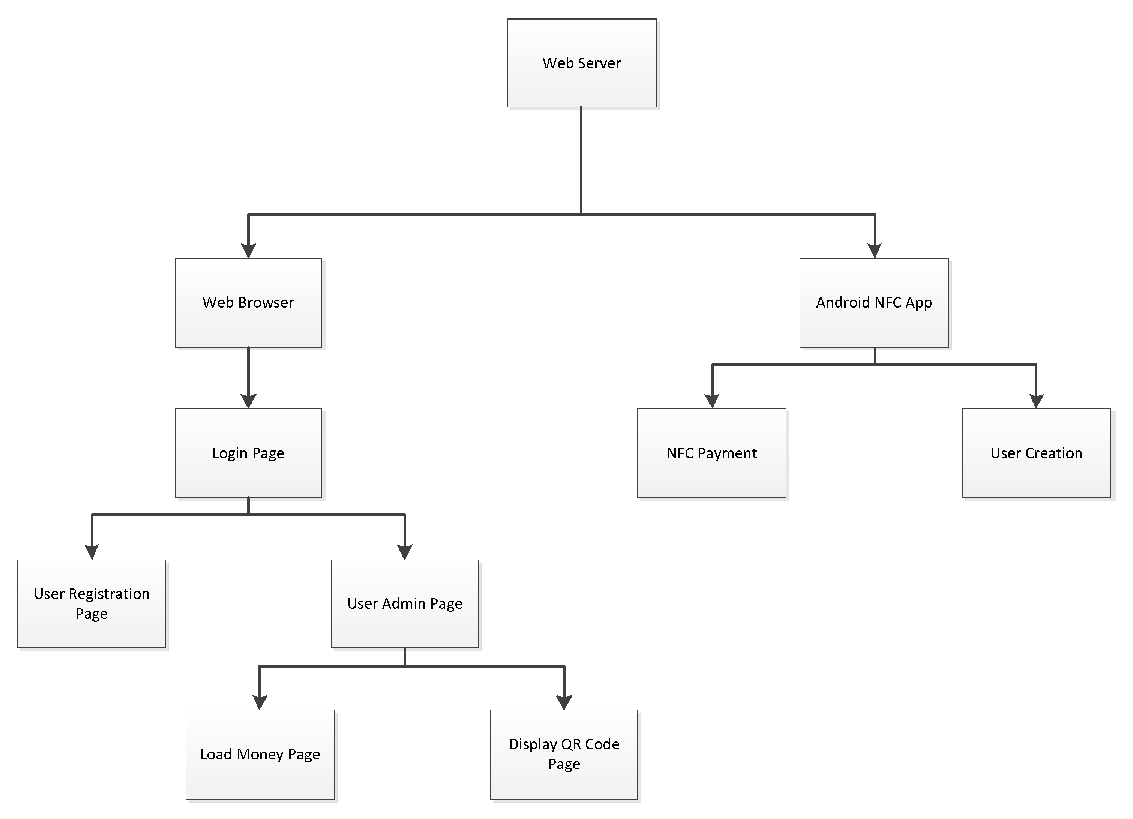
\includegraphics[clip=true, trim = 50 260 0 90,
 scale=0.7]{website_structure}
 \caption{The web server application structure.}
 \label{fig:website-apps}
\end{figure}

\subsubsection{display\_qrcode}

This application forms the core of the Quick Response Code (QR Code) payment handling
part of the server. See Fig. \ref{fig:disp-qrcode} for the process flow of
this application.

\begin{figure}
 \centering 
 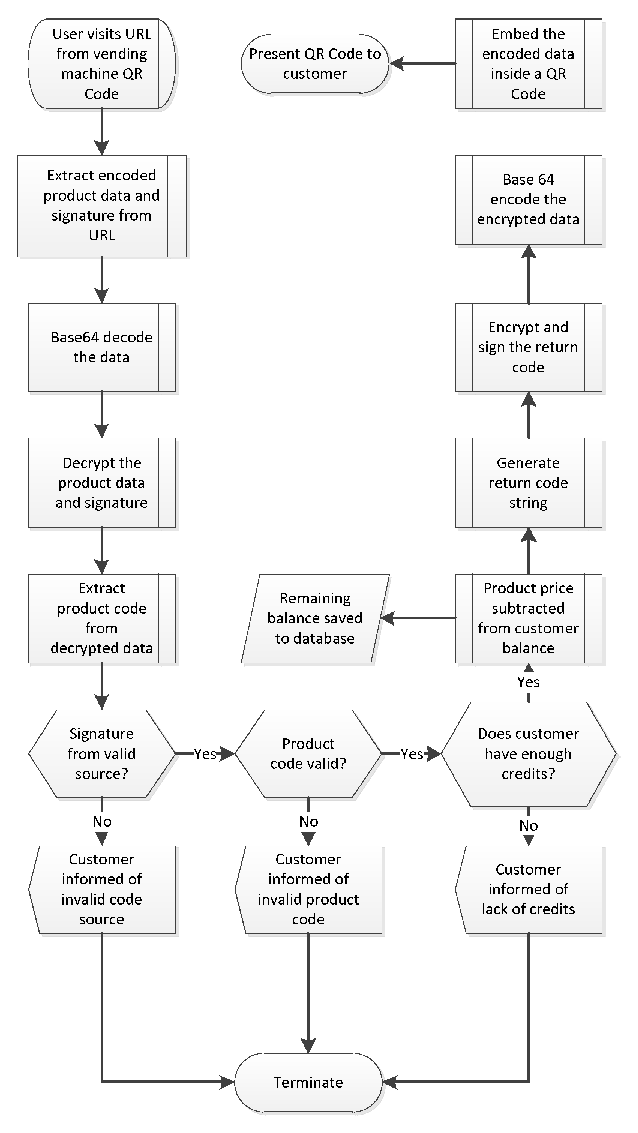
\includegraphics[clip=true, trim = 0 250 0 120,
 scale=0.7]{qrcode_processflow_server_bak}
 \caption{The display\_qrcode application process flow.} 
 \label{fig:disp-qrcode}
\end{figure}

Fig. \ref{fig:disp-qrcode} shows that the application first extracts the code
containing the product code and VM's signature from the Uniform
Resource Locator (URL) that the customer requested with his cellphone's web
browser. The application then proceeds to decode the product code from its base64
encoded format.

After successfully decoding the data, the application proceeds to decrypt the data and
signature with the ElGamal algorithm using the server's private key and the
VM's public key. Afterwards, following the security code scheme described in Sec.
\ref{sec:security-code-scheme}, it extracts the product code and challenge from the
decrypted string.

The application then checks to see whether the signature comes from a valid source (i.e.
one of the VMs using this system), whether the product code is
valid (i.e. the product is in the database) and whether the customer has enough
credits available. If either of these checks return false,
an error message is shown to the customer explaining what went wrong
and what the customer should do next.

If the checks were passed, the application proceeds to subtract the product cost from
the user's remaining balance. Following the security code scheme, the application then
generates the correct return code, encrypts and signs it with the vending
machine's public key and the server's private key, and encodes it in base64.
After this is completed, the application embeds this data into a QR Code, which is
displayed on the customer's cellphone screen.

\subsubsection{load\_money}

This application allows the customer to load money onto his account. At the moment it
makes use of faux money, meaning that the money loaded has no real-world value.
The customer can load a maximum of R1000.00 at a time onto his account. See Fig.
\ref{fig:load-money} for the process flow of this application.

\begin{figure}
 \centering 
 \includegraphics[clip=true, trim = 0 580 100 70,
 scale=0.7]{load_money}
 \caption{The load\_money application process flow.}
 \label{fig:load-money}
\end{figure}

\subsubsection{nfc}
\label{sec:app-nfc}

This application forms the core of the NFC payment handling part of the server. See Fig.
\ref{fig:nfc-process} for a detailed process flow diagram.

\begin{figure}
 \centering 
 \includegraphics[clip=true, trim = 0 220 50 150,
 scale=0.7]{nfc_processflow_bak}
 \caption{The NFC application process flow.}
 \label{fig:nfc-process}
\end{figure}

Fig. \ref{fig:nfc-process} shows that the server first extracts the encrypted
customer login details and product code from the NFC application's URL request. These
codes are then decoded and decrypted using the RSA algorithm and the server's private key.

The user login details are then checked and verified using the server's user database. If this
check fails, the customer is given an error message and is asked to create a user profile.
If the check is passed, the server then checks to see if the customer has enough money
loaded onto his account. If this check fails, the customer is informed of his lack of
funds and is instructed to load more money. If the check is passed, the server subtracts
the product cost from the customer's balance and encrypts and encodes a confirmation
code, according to the security code scheme specified in Sec.
\ref{sec:security-code-scheme}. This code is then sent to the NFC application.

\subsubsection{nfc\_add\_user}
\label{sec:nfc-add-user}

This application allows a customer using the NFC application to create a user profile for
himself. The server extracts the customer's login details from the URL request that the
NFC application sends to the server. These details are then saved to the database and is immediately available to be used by the new
customer. 

\subsubsection{register}

This application allows a new customer to register a new user profile with an internet
browser. This application is only accessible by a web browser and not by the NFC
application. However, a user registered with this application will be able to use the
same login details for the NFC application, and vice versa.

The application presents the user with a simple registration page which asks for a user
name, email and password. Using Django's built-in form support, the server handles the
POST request that is generated when the customer presses the `Continue' button. When this
is done, the customer's login details contained within the POST request is extracted and
saved into the user database.

\section{Vending Machine Program}

The vending machine's program runs the VM. It is responsible for
allowing the customer to select a product, to create a QR Code that redirects
the customer to the web server, to scan the customer's response QR Code, to
scan the customer's NFC/RFID request and to dispense the product after a successful
transaction.

The whole program is based on Python and designed to be used by a Raspberry Pi
microcomputer. To simplify the program, it is split into separate subprograms. These
subprograms, called scripts, are discussed in this section. The complete
program structure and its inter-script interfaces can be seen in Fig.
\ref{fig:vm_prog_strcture}. The source code is available on
github.com/jayceelock/vending\_prog and in the project file. 

\begin{figure}
 \centering 
 \includegraphics[clip=true, trim = 120 370 0 50,
 scale=0.7]{vending_machine_program_structure}
 \caption{The vending machine's program structure.}
 \label{fig:vm_prog_strcture}
\end{figure}

\subsection{User Interface}

To allow the customer to select a product, a Graphical User Interface (GUI) was
created. The GUI was made using the WX Python GUI toolkit
[\cite{website:wx-python}].
See Fig. \ref{fig:gui-screenshot} for a screenshot of the
GUI.

\begin{figure}
 \centering 
 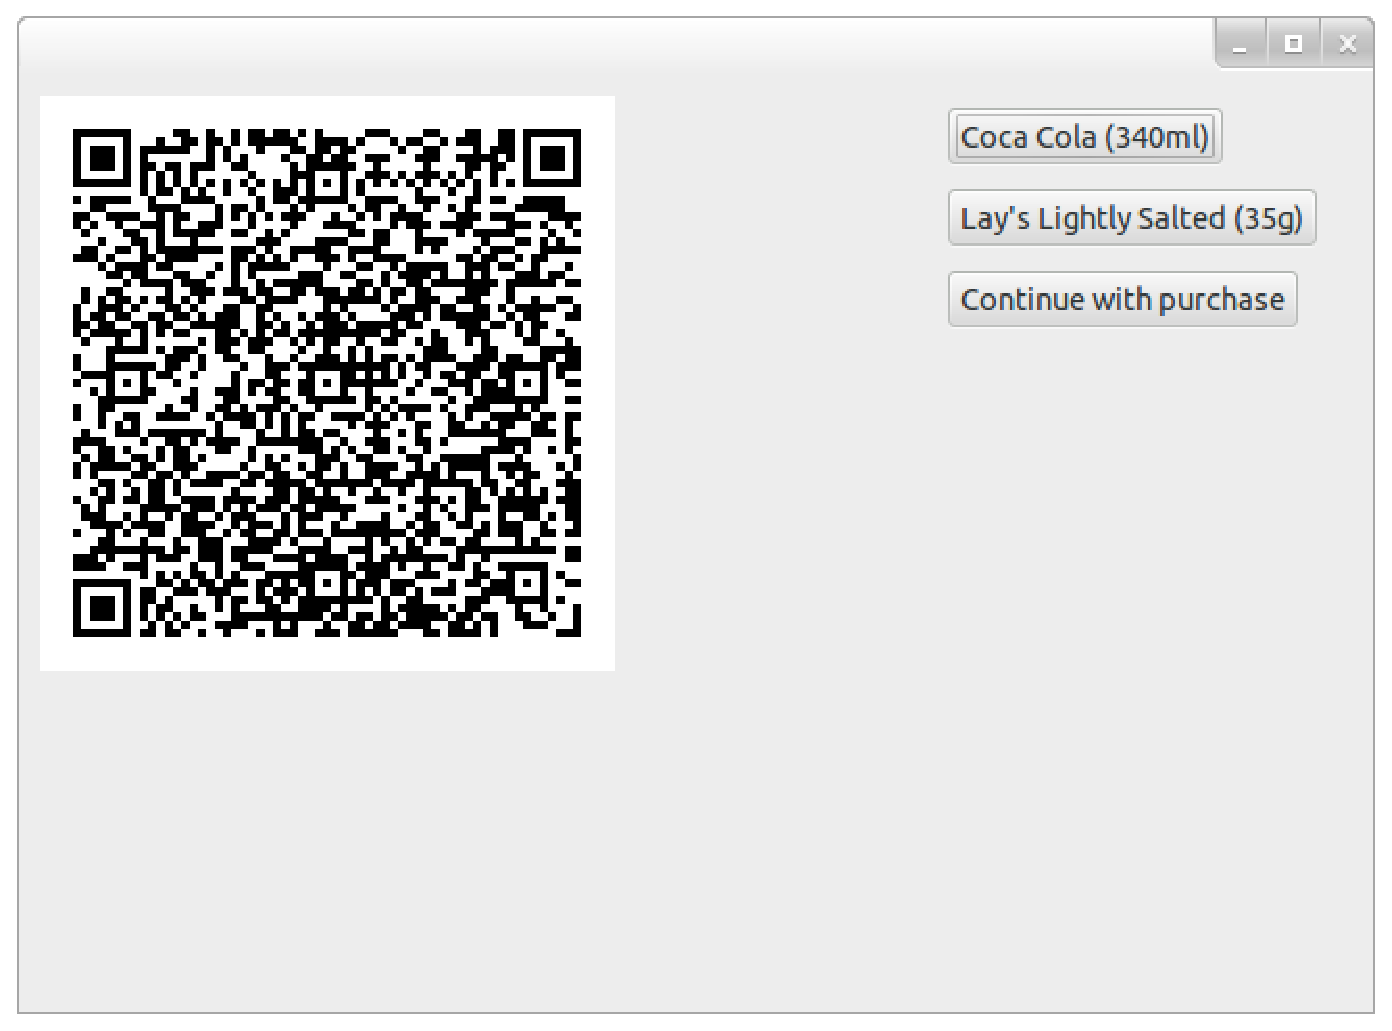
\includegraphics[clip = true, trim = 190 370 0 350, scale=2]{gui_screenshot}
 \caption{A screenshot of the user interface.}
 \label{fig:gui-screenshot}
\end{figure}

As can be seen from Fig. \ref{fig:vm_prog_strcture}, the GUI script is
responsible for calling the encryption script and the QR Code generation script.
It is also responsible for displaying the QR Code, to handle transactions from
the Android NFC application and to activate the correct motor inside the vending
machine. 

\subsection{Generating a Product Code}

After the customer selects which product to buy from the GUI, the
encrypt\_elgamal script is called. This script is responsible for generating the
random hex character string, in accordance with the security scheme described in
Sec. \ref{sec:security-code-scheme}, encrypting, signing and encoding the
string in base64 and embedding the random string inside a URL that points to the web
server. This URL is then sent to the generate\_qrcode script described in Sec.
\ref{sec:gen-qrcode}. See Fig. \ref{fig:gen-prod-code-processflow} for a detailed process
flow diagram.

\begin{figure}
 \centering 
 \includegraphics[clip=true, trim = 0 570 50 120, scale=0.7]{gui_processflow}
 \caption{The GUI process flow.}
 \label{fig:gen-prod-code-processflow}
\end{figure}

\subsection{Generating a QR Code}
\label{sec:gen-qrcode}

After the encrypt\_elgamal script has been run, the generate\_qrcode script is
called. This script is responsible for embedding the URL received from the
encrypt\_elgamal script into a QR Code. This is done by using a qrcode module
for Python, called qrcode [\cite{website:qrcode-generator}].

\subsection{Reading a QR Code}

After the customer has received his verification QR Code from the server, the customer
may presses `Continue with purchase' button. When this is done, the read\_qrcode script is
run. This script is responsible for reading the customer's QR Code via a webcam,
extracting the data from the scanned image, decrypting the data and verifying the
transaction. See Fig. \ref{fig:read-qrcode-processflow} for the process flow diagram.

\begin{figure}
 \centering 
 \includegraphics[clip=true, trim = 0 400 50 80, scale=0.75]{read_qrcode_processflow}
 \caption{The generate\_qrcode script process flow.}
 \label{fig:read-qrcode-processflow}
\end{figure}

As seen from Fig. \ref{fig:read-qrcode-processflow}, as soon as the `Continue
with purchase' button is pressed, a ZBar image processor is created
which scans a webcam video feed for a QR Code. The image processor runs until the user
cancels it or it scans a QR Code. 

After the ZBar processor has scanned a QR Code, it sends the retrieved data to
be decrypted and verified with the ElGamal algorithm, using the VM's
private key and the server's public key. If the signature is valid and the data
contains a valid response and product code, the script activates the correct
motor and the customer receives his product. 

\subsection{Near Field Communication}

If the customer opts to purchase a product with the Android NFC application, the NFC
script is run. This script is based on an example script included in the nfcpy package and is written by nfcpy's creator, Stephen
Tiedemann [\cite{website:nfcpy}]. This example script, called snep\_test\_server.py,
connects the Pi to the NFC controller chip, polls the chip for a Simple NFC Data Exchange Format
Exchange Protocol (SNEP) message, and when a SNEP message is read, it extracts the data
in the message and presents it to the programmer for further processing and manipulation.
This script allows the VM to extract SNEP messages from any source that
follows the NFC Forum's standards [\cite{website:nfc-forum}]. For this project, an
Android application was written specifically for this purpose.

After the data is extracted from the NFC source, the script decrypts the data
using the RSA algorithm and the VM's private key. The vending
machine then checks the NFC message's response code. If the response code is valid, the
script then activates the correct motor to dispense the product to the customer.

\subsection{Radio Field Identification}

This module allows for a purchase to take place using a Radio Field
Identification (RFID) card, such as a SU card. It is based on an example script
from the libnfc module. The transaction process and its shortcomings are
discussed in Sec. \ref{sec:su-card}

It works by using the libnfc module to scan for a RFID
card. When a card is detected, it extracts the card's Unique Identification (UID)
number. If the UID number is present in the VM's code, the script activates the
correct motor and the customer receives his product. 

\section{Android Application}
\label{sec:nfc-android-app}

An Android NFC application was made for this project. It allows a customer to buy a
product from the application's product menu and to complete the purchase by tapping
his phone against the VM's NFC receiver.

The application is divided up into three activities (Android's technical term for what
is essentially a different window of the application). These activities, their design and
significance are discussed in this section. See Fig. \ref{fig:nfc_app_structure} for a
diagram of the application's inter-activity interactions.

The source code is available from github.com/jayceelock/nfcpay6 and in the
project file.

\begin{figure}
 \centering 
 \includegraphics[clip = true, trim = 40 410 0 20,
 scale=0.7]{app_structure}
 \caption{The Android NFC application structure.}
 \label{fig:nfc_app_structure}
\end{figure}

\subsection{Welcome Screen}

This activity is called when the application is opened. This
activity's process flow can be seen in Fig. \ref{fig:app-welcomescreen}.
Fig. \ref{fig:welcomescreen-screenshot} shows a screenshot of the welcome
screen.

\begin{figure}
 \centering 
 \includegraphics[clip = true, trim = 30 490 0 150,
 scale=0.75]{welcome_screen_processflow}
 \caption{The Android NFC application welcome screen.}
 \label{fig:app-welcomescreen}
\end{figure}

\begin{figure}
 \centering 
 \includegraphics[clip = true, trim = 0 620 0 60,
 scale=0.2]{welcome_screenshot}
 \caption{A screenshot of the application's welcome screen.}
 \label{fig:welcomescreen-screenshot}
\end{figure}

As seen from Fig. \ref{fig:app-welcomescreen}, the
activity first checks to see whether it is the first time the user opens the
application. If it is not, the activity goes on to the Main Activity. Otherwise, it allows
the user to either sign in with an existing profile or create a new one.

When the user signs into an existing profile, the login details he provides
is stored in a database inside the application. When this is done, it
makes the login information persistent throughout the lifetime of the application. These
details are also saved into an application-wide variable. This variable is used to make
the application more efficient by not having to read the database as often. This variable
is only active while the application is running in the foreground or background. The
login details saved here are used later by the application's other activities.

If the user checks the `New user' checkbox, the application the data is
still saved to the database and the app-wide variable, but the
applications also encrypts and embeds the user's login information into a URL.
The application then sends this URL to the server, which then decrypts and saves
the data to the user database. See Sec. \ref{sec:nfc-add-user} for more detail on
the server activity.

After this has been done, the Main Activity is launched. 

\subsection{Main Activity}

The main activity is the activity which is responsible for encrypting and
sending the purchase requests to the web server, receiving and decrypting
the purchase approval codes and sending the NFC messages to the VM's
NFC receiver. See Fig. \ref{fig:main-activity} for a process flow diagram
and Fig. \ref{fig:main-activity-screenshot} for a screenshot of this activity.

This activity is based on example code for NFC usage from Google
[\cite{website:google-nfc}] and the encryption and base64 encoding section is
based on an encryption tutorial by tibi [\cite{article:android-encryption}].

\begin{figure}
 \centering 
 \includegraphics[clip = true, trim = 0 430 50 70,
 scale=0.7]{app_main_processflow}
 \caption{The process flow of the Main activity.}
 \label{fig:main-activity}
\end{figure}

\begin{figure}
 \centering 
 \includegraphics[clip = true, trim = 0 850 0 60,
 scale=0.2]{main_screenshot}
 \caption{A screenshot of the application's main activity.}
 \label{fig:main-activity-screenshot}
\end{figure}

As seen from Fig. \ref{fig:main-activity-screenshot}, the activity presents
the user with a list of products. When the user selects a product to buy, the
activity forms a data string by adding the product code, the user's login
name and password together. This data string is then encrypted with the
server's public key and then encoded to base64. This encoded string
is then embedded inside a URL which points to the web server. 

The activity then requests this URL in the application's background, which prompts the
server to process the transaction (see Sec. \ref{sec:app-nfc} for more details on the
server's NFC processes). The server then tells the activity if the transaction
has been approved or denied. If it has been denied, the user is informed what was wrong. 
If it is approved, the activity activates the cellphone's NFC antenna which transmits an
encrypted approval message to the VM's NFC receiver.

\subsection{Change User Settings}

The Change User Settings activity allows the user to change his login
details that are saved in the database and the application-wide variable. See Fig.
\ref{fig:change-user-settings} for a process flow diagram for this
activity. Fig. \ref{fig:change-settings-screenshot} shows a screenshot of this
activity.

\begin{figure}
 \centering 
 \includegraphics[clip = true, trim = 0 680 0 20,
 scale=0.7]{change_settings_processflow}
 \caption{The process flow of the Change Settings activity.}
 \label{fig:change-user-settings}
\end{figure}

\begin{figure}
 \centering 
 \includegraphics[clip = true, trim = 0 680 0 60,
 scale=0.2]{settings_screenshot}
 \caption{A screenshot of the application's change settings activity.}
 \label{fig:change-settings-screenshot}
\end{figure}

When the application enters this activity, it prompts the user to enter his user
name and password. When the user presses the `continue button', the old database
entry and application-wide variable is overwritten with the new values the user entered.
The details stored on the server's database is not affected, however.
\chapter{Hardware Detail Design}
\label{chap:5}

This chapter gives a detailed discussion on the hardware design and
configuration of this system. This includes the relay switching circuit, the
motor and coil design and the NFC chip configuration.

See Appendix \ref{app:d} for a schematic layout of the hardware and their
connections.

\section{Relay Switch Circuit}
\label{sec:detail-switch}

As explained in Sec. \ref{sec:relay-switch} on p.\pageref{sec:relay-switch}, a relay
switch [\cite{manual:relay-specs}], in conjunction with a 2N2222
Bipolar Junction Transistor (BJT) [\cite{maunual:transistor-datasheet}], is used
by the Raspberry Pi to control the motor. See Fig.
\ref{fig:relay-switch} for the circuit diagram.

\begin{figure}
\centering
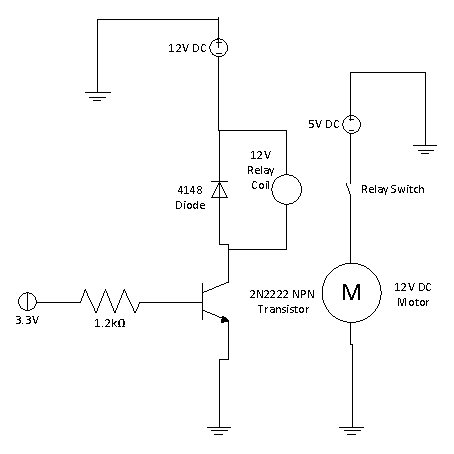
\includegraphics[clip = true, trim = 70 640 0 70, scale=1.2]{relay_switch}
\caption{12 V relay transistor switch.}
\label{fig:relay-switch}
\end{figure}

For the following equations, P$_r$ and V$_r$ is the power dissipation in the relay coil
and voltage across the relay coil, $\beta$ is the BJT current amplification, V$_p$ and
I$_p$ is the voltage and current supply from a Raspberry Pi's GPIO pin and I$_b$ and
R$_b$ is the BJT's base current and resistor.

The relevant  parameters for these components are [\cite{manual:relay-specs},
\cite{maunual:transistor-datasheet}]:

\[ \mathrm{\ P_{r}} = 0.36\mathrm{\ W}\]
\[ \mathrm{\ V_{r}} = 12\mathrm{\ V}\]
\[ \mathrm{\ \beta} \approx 10\]
\[ \mathrm{\ V_{p}} = 3.3\mathrm{\ V}\]

From the relay's power dissipation and voltage, its current draw is found by

\[
\mathrm{\ I_{r}} = \frac{\mathrm{\ P_{r}}}{\mathrm{\ V_{r}}}
\]

which gives a current draw of

\[
\mathrm{\ I_{r}} = 0.03\mathrm{\ A}
\]

Taking the BJT's current amplification as roughly 10, as recommended by the
BJT's datasheet [\cite{maunual:transistor-datasheet}], the current draw from the
Pi to the base of the BJT is given by

\[
\mathrm{\ I_{b}} = \frac{\mathrm{\ I_{r}}}{\beta}
\]

This gives a current draw of

\[
\mathrm{\ I_{b}} = 3\mathrm{\ mA}
\]

The maximum allowable current draw from a GPIO pin is 16 mA
[\cite{website:gpio-specs}], though this is not recommended as the Pi does not
have any current limiting or over-current protection hardware. A current draw of 5mA per
pin is recommended by the Pi's manufacturers [\cite{website:gpio-specs}]. Therefore, a
current draw of 3 mA is completely safe.

To limit the current draw from the Pi, a base resistor must be added between the Pi's GPIO pin
and the BJT's base. With a current draw of 3 mA and a voltage of 3.3 V, the
resistor size is found by using Ohm's law:

\[
\mathrm{\ R_{b}} = \frac{\mathrm{\ V_{p}}}{\mathrm{\ I_{p}}}
\]

which gives

\[
\mathrm{\ R_{b}} = 1.1\mathrm{\ k\Omega}
\]

To prevent voltage spikes from the Pi's GPIO's from supplying to much current, a
further 10\% was added to the resistor size. This gives a resistor size of

\[\mathrm{\ R_{b}} = 1.2\mathrm{\ k\Omega}\]

which draws a current of 

\[\mathrm{\ I_{b}} = 2.75\mathrm{\ mA} \]

which is still enough to activate the relay's coil and turn the motor on. 

\section{NFC Chip}

The Near Field Communication (NFC) chip used, is the Adafruit NFC shield for an
Arduino Uno microcontroller [\cite{website:adafruit-nfc}]. See Sec.
\ref{sec:nfc-controller} on p.\pageref{sec:nfc-controller} for more details
on the controller.

The shield was designed and built to be used by an Arduino Uno microcontroller.
Therefore, some modification to the chip's connections had to be made before it
was able to communicate with the Pi. By default, the chip was made to communicate with an
Arduino using the Inter Integrated Circuit (i$^2$c) communication protocol. However, the
component manufacturers have added connection pads to the chip that, when shorted, allows
the chip to communicate via Serial Peripheral Interface (SPI) or Transistor
Transistor Login (TTL). The libnfc library is currently only configured to allow
communication via an Universal Asynchronous Receiver Transmitter (UART). Therefore, the
chip was modified to communicate via its TTL interface, which is compatible with the Pi's
UART interface. 

See Appendix \ref{app:nfc-chip-config} for detailed explanation on this
configuration process and also how the libnfc library was built and compiled. 

\section{Vending Machine Unit}

A small VM unit was constructed for demonstration purposes. It is
designed to house all the VM components, i.e. the two DC motors,
the two coils, the Raspberry Pi central controller, the NFC shield and the
webcam.

Four 10 mm vent holes were added at the sides to improve air circulation
and to provide external wire access, while a larger 60 mm vent hole was also
added to allow for an external 60 mm desktop computer fan to be added at a
later stage.

The unit is made from 1.6 mm thick mild steel and the components were cut and
bent by Fabrinox, Paarl and welded together by the Electrical and Electronic
Engineering Department of Stellenbosch University's workshop.

See Fig. \ref{fig:vm-actual} in Appendix \ref{app:vm-tekeninge} for a picture of the
complete VM unit with the two DC motor inserted. See Appendix \ref{app:vm-tekeninge} for
detailed design drawings of the VM unit.

\section{Webcam}

As discussed in Sec. \ref{sec:webcam}, a Sony PS2 Eye Toy  webcam was
attached to the Raspberry Pi. This allows the VM to scan a live
video feed for a QR Code. It is already compatible with the Raspberry Pi and
therefore requires minimal configuration to begin working.

It is important to note that a Raspbian version from early 2013 was used on the
Raspberry Pi. It was found that the latest Raspbian distributions have an
unknown bug in its Video4Linux video drivers which causes the EyeToy to
work incorrectly. Furthermore, the camera needs to be plugged into a Universal Serial Bus
(USB) port on the Pi itself and not into an external USB hub. This is done to prevent
hardware timing issues that are introduced when a USB hub is used.

\section{Motor and Coil}

The VM dispenses products by activating a motor that turns a coil
loaded with a product. This turning motion causes a product to move along the
coil in an Archimedean screw-like manner until it falls off at the end of the
coil. 

In the demonstration VM, two coils are used. The coils are made
from 2.5 mm thick galvanised iron wire. The coil diameter is 50 mm and has a
longitudinal pitch of 20 mm. 

It is important to only activate the motor for one turn of the coil to
ensure that only one product is dispensed per completed transaction. This is
currently being done by only activating a motor for a set amount of time. To
determine this time, it was required that the speed of the motor be
determined for a given supply voltage. The motors that are used are 12 V DC motors made
by Faulhaber [\cite{manual:dc-motors}] coupled with a 14:1 speed gearbox
[\cite{manual:gearbox}].

For the following calculations, V$_o$, I and R are the motor supply voltage, current and
terminal resistance, V$_e$ is the back-Electromotive Force (EMF) voltage, $\omega$ is
the motor speed and k$_e$ is the Back-EMF constant.

The following equation gives the relationship between a DC motor's supply
voltage and its back-Electromotive Force (EMF) [\cite{article:motor-calc}].

\[ \mathrm{V}_o = \mathrm{IR} + \mathrm{V}_e\]

The back-EMF is proportional to the rotational speed of the motor. Therefore,
the V$_e$ term can be taken as

\[ \mathrm{V}_e = \mathrm{k}_e\omega\]

which gives the following equation

\begin{equation}
 \label{eq:motor}
 \mathrm{V}_o = \mathrm{IR} + \mathrm{k}_e\omega
\end{equation}

The IR term is taken as constant, since the torque load on the motor stays the constant.
From the motor's datasheets and usage tests, the I, R and k$_e$ terms were
determined to have the following values:

\[\mathrm{I} = 0.35\mathrm{\ A}\]
\[\mathrm{R} = 0.41\mathrm{\ \Omega}\]
\[ \mathrm{k}_e = 2 \mathrm{\ mV/rpm}\]

Using these values, and setting the input voltage as 3.3 V in equation
\ref{eq:motor}, the motor's speed was determined to be 113 RPM. Therefore, to
complete a single revolution, the motor may only be activated for 0.53 seconds. 

This is not the most effective method, however, because the errors in the system
accumulate over time. In time, these errors may lead incorrect product
dispensing. 

To improve this, a proximity sensor may be added onto the coil and onto the
VM wall. This sensor can be connected to and be controlled by the
Raspberry Pi and would be activated every time the coil completes one
revolution. When the sensor is triggered, the Pi will then know that exactly
one revolution has been completed and stop the motor. This will stop any errors
from accumulating over time and make the VM more reliable. 

\chapter{System Tests}

In this chapter, the tests  conducted to measure how well the system measures to the
original goals and objectives set out in Section \ref{chap:1}. 

The tests conducted are the voltage and current limits of the relay switches and user
stories where scenarios are created and the response of the system is given. 

\section{Transistor Switch}

MOET NOG GEDOEN WORD

\subsection{Current and Voltage Limits}

MOET NOG GEDOEN WORD

\section{User Tests}

The functionality of the system is tested by exposing it to different user scenarios and
seeing what the outcome is. These tests are performed and discussed in this section.

\subsection{Test 1}

In this user story, the customer decides to pay with a Quick Response Code (QR Code).
He/she does not yet have a user account on the database and has no credits laoded. Figure
\ref{fig:test1} shows the user story. 

The process is as follows: The user first selects which product to buy from the Raspberry
Pi's User Interface (GUI). The Pi then generates a Quick Response Code (QR Code) that the
user scans with any barcode scanning application. The Universal Resource Locator (URL)
embedded in the QR Code then takes the customer to a web page located on the server. 

Not having a user account, the user clicks on the lick to create a new user profile. After
entering valid user information, the customer is returned to the login  page where he/she
can log in with his/her new login credentials. 

After logging in, the server displays to the customer that he/she does not yet have any
credits loaded onto his/her account. The customer then goes to the load credit page where
they load some money. When this is done, the server displays a confirmation QR Code on
the customer's cell phone screen, verifying the transaction.

The customer then presses the continue button on the GUI, which starts scanning the web
cam feed for the customer's QR Code. After this is done, the Pi activates the correct
motor and dispenses the product.

\begin{figure}
 \centering 
 \includegraphics[clip=true, trim = 0 470 0 50,
 scale=0.7]{user_story_1}
 \caption{The first user scenario}
 \label{fig:test1}
\end{figure}

\subsection{Test 2}

In this scenario, a customer tries to use a QR Code from a previous transaction. Figure
\ref{fig:test2} shows the user story.

To begin, the customer selects a product to buy, after which the Raspberry Pi displays a
QR Code. However, instead of scanning the QR Code and paying for a new product, the
customer tries to use an old QR Code that the server sent him/her after a successful
transaction previously. 

The customer tells the Raspberry Pi to scan his/her old QR Code. The Raspberry Pi does
this, but the old QR Code does not contain a valid response to the Raspberry Pi's
challenge. Therefore, the transaction is valid and the customer is informed of his/her
invalid QR Code.

\begin{figure}
 \centering 
 \includegraphics[clip=true, trim = 0 620 0 50,
 scale=0.7]{user_story_2}
 \caption{The second user scenario}
 \label{fig:test2}
\end{figure}

\subsection{Test 3}

In this scenario, the user opts to buy a product using the Android Near Field
Communication (NFC) app. However, a new user profile must first be created. The user story
can be seen in Figure \ref{fig:test3}.

After the user opens the app, he/she is presented with a login screen. The user enters
his/her login credentials and checks the box that confirms that he/she is a new user. The
app then contacts the server with a user creation request. Provided that the username is
not already in use, the server sends the app a confirmation.

The app then returns the user to the main menu where the user can pick a product to buy.
After picking a product, the app contacts the server with a purchase request. If the
transaction is successful, the server sends the app a confirmation code which the app 
transmits via the cell phone's NFC antenna. 

The user then swipes his/her phone across the vending machines NFC receiver. The vending
machine then activates the motor and the user receives his/her product. 

\begin{figure}
 \centering 
 \includegraphics[clip=true, trim = 0 500 0 50,
 scale=0.7]{user_story_3}
 \caption{The third user scenario}
 \label{fig:test3}
\end{figure}

\appendix%===========================================================

%\chapter{Vending Machine Drawing}
\label{app:vm-tekeninge}

\begin{figure}
 \centering 
 \includegraphics[clip=true, trim = 80 180 150 200,
 scale=0.7]{complete_vm}
 \caption{The complete vending machine unit.}
 \label{fig:vm-actual}
\end{figure}
%\chapter{dude}
%\include{App-B}
%\include{App-C}

\backmatter%=========================================================

\bibliography{bibliography}

\end{document}